\section{AC/DC theory}

\begin{frame}{}
    \tableofcontents[currentsection]
\end{frame}

\subsection{Grid basics}
\begin{frame}{What is a power grid?}

\begin{figure}[!htb]
    \centering
    \begin{tikzpicture}[european, scale=0.9]

        % 0. Draw nodes
        \node(1) at (-0.2, 0) {1};
        \node(2) at (1.8, -2) {2};
        \node(3) at (5.0, -2) {3};
        \node(4) at (5.8, 0) {4};
        \node(5) at (4.0, 0) {5};
        \node(6) at (4.0, 1.5) {6};

        % 1. Draw buses (Passive lines in blue)
        \draw[line width=0.1cm] (0, 0) to [short] (0.8, 0);
        \draw[line width=0.1cm] (2, -2) to [short] (2.8, -2);
        \draw[line width=0.1cm] (6, 0) to [short] (6.8, 0);
        \draw[line width=0.1cm] (3, 0) to [short] (3.8, 0);
        \draw[line width=0.1cm] (4, -2) to [short] (4.8, -2);
        \draw[line width=0.1cm] (3, 1.5) to [short] (3.8, 1.5);

        % 2. Draw transformers (red circles)
        \draw[thick, black] (3.4, 0.65) circle (0.2cm);
        \draw[thick, black] (3.4, 0.85) circle (0.2cm);

        % 3. Draw generators with additional busbars
        \draw (0.4, 0.75) to [/tikz/circuitikz/bipoles/length=25pt, sinusoidal voltage source] (0.4, 0.25);
        \draw (0.4, 0.25) to [short] (0.4, 0); 

        \draw (2.4, -2.25) to [/tikz/circuitikz/bipoles/length=25pt, sinusoidal voltage source] (2.4, -2.75);
        \draw (2.4, -2.25) to [short] (2.4, -2.0); 

        \draw (4.4, -2.25) to [/tikz/circuitikz/bipoles/length=25pt, sinusoidal voltage source] (4.4, -2.75);
        \draw (4.4, -2.25) to [short] (4.4, -2.0); 

        % 4. Draw loads
        \draw (2.1, -2) to [short] (2.1, -2.2);
        \draw[-{Latex[scale=1.5]}] (2.1,-2.2) -- (1.3,-2.2);

        \draw (4.7, -2) to [short] (4.7, -2.2);
        \draw[-{Latex[scale=1.5]}] (4.7,-2.2) -- (5.5,-2.2);

        \draw (6.8, 0) to [short] (7.0, 0);
        \draw[-{Latex[scale=1.5]}] (7.0, 0) -- (7.0, -0.8);

        \draw (3.1, 0) to [short] (3.1, 0.2);
        \draw[-{Latex[scale=1.5]}] (3.1, 0.2) -- (2.3, 0.2);

        \draw (3.7, 1.5) to [short] (3.7, 1.7);
        \draw[-{Latex[scale=1.5]}] (3.7, 1.7) -- (4.5, 1.7);

        % Draw lines (Passive lines in blue)
        \draw[black] (0.4, 0) to [short] (0.4, -0.2);
        \draw[black] (2.2, -2) to [short] (2.2, -1.8);
        \draw[black] (0.4, -0.2) to [short] (2.2, -1.8);

        \draw[black] (0.6, 0) to [short] (0.6, -0.2);
        \draw[black] (3.2, 0) to [short] (3.2, -0.2);
        \draw[black] (0.6, -0.2) to [short] (3.2, -0.2);

        \draw[black] (3.4, 0) to [short] (3.4, -0.2);
        \draw[black] (2.4, -2) to [short] (2.4, -1.8);
        \draw[black] (3.4, -0.2) to [short] (2.4, -1.8);

        \draw[black] (2.6, -2) to [short] (2.6, -2.2);
        \draw[black] (4.2, -2) to [short] (4.2, -2.2);
        \draw[black] (2.6, -2.2) to [short] (4.2, -2.2);

        \draw[black] (2.6, -2) to [short] (2.6, -1.8);
        \draw[black] (6.4, 0) to [short] (6.4, -0.2);
        \draw[black] (2.6, -1.8) to [short] (6.4, -0.2);

        \draw[black] (3.6, 0) to [short] (3.6, -0.2);
        \draw[black] (6.2, 0) to [short] (6.2, -0.2);
        \draw[black] (3.6, -0.2) to [short] (6.2, -0.2);

        \draw[black] (4.4, -2) to [short] (4.4, -1.8);
        \draw[black] (6.6, 0) to [short] (6.6, -0.2);
        \draw[black] (4.4, -1.8) to [short] (6.6, -0.2);

        \draw[black] (3.4, 0) to [short] (3.4, 0.45);
        \draw[black] (3.4, 1.05) to [short] (3.4, 1.5);
    \end{tikzpicture}
    \caption{Example grid showing buses linked through branches.}
    \label{fig:14bus}
\end{figure}

    A grid is modeled as an undirected graph the set of buses (nodes) are connected to each other by the set of branches (edges):
    \begin{itemize}
        \item \textbf{Buses}: Represent the points in the network where generation, load, or interconnections occur.
        \item \textbf{Branches}: Power lines, transformers and converters, which can be passive or controllable.
    \end{itemize}
\end{frame}



\begin{frame}{Grid of grids}
    \begin{figure}[H]
    \centering
    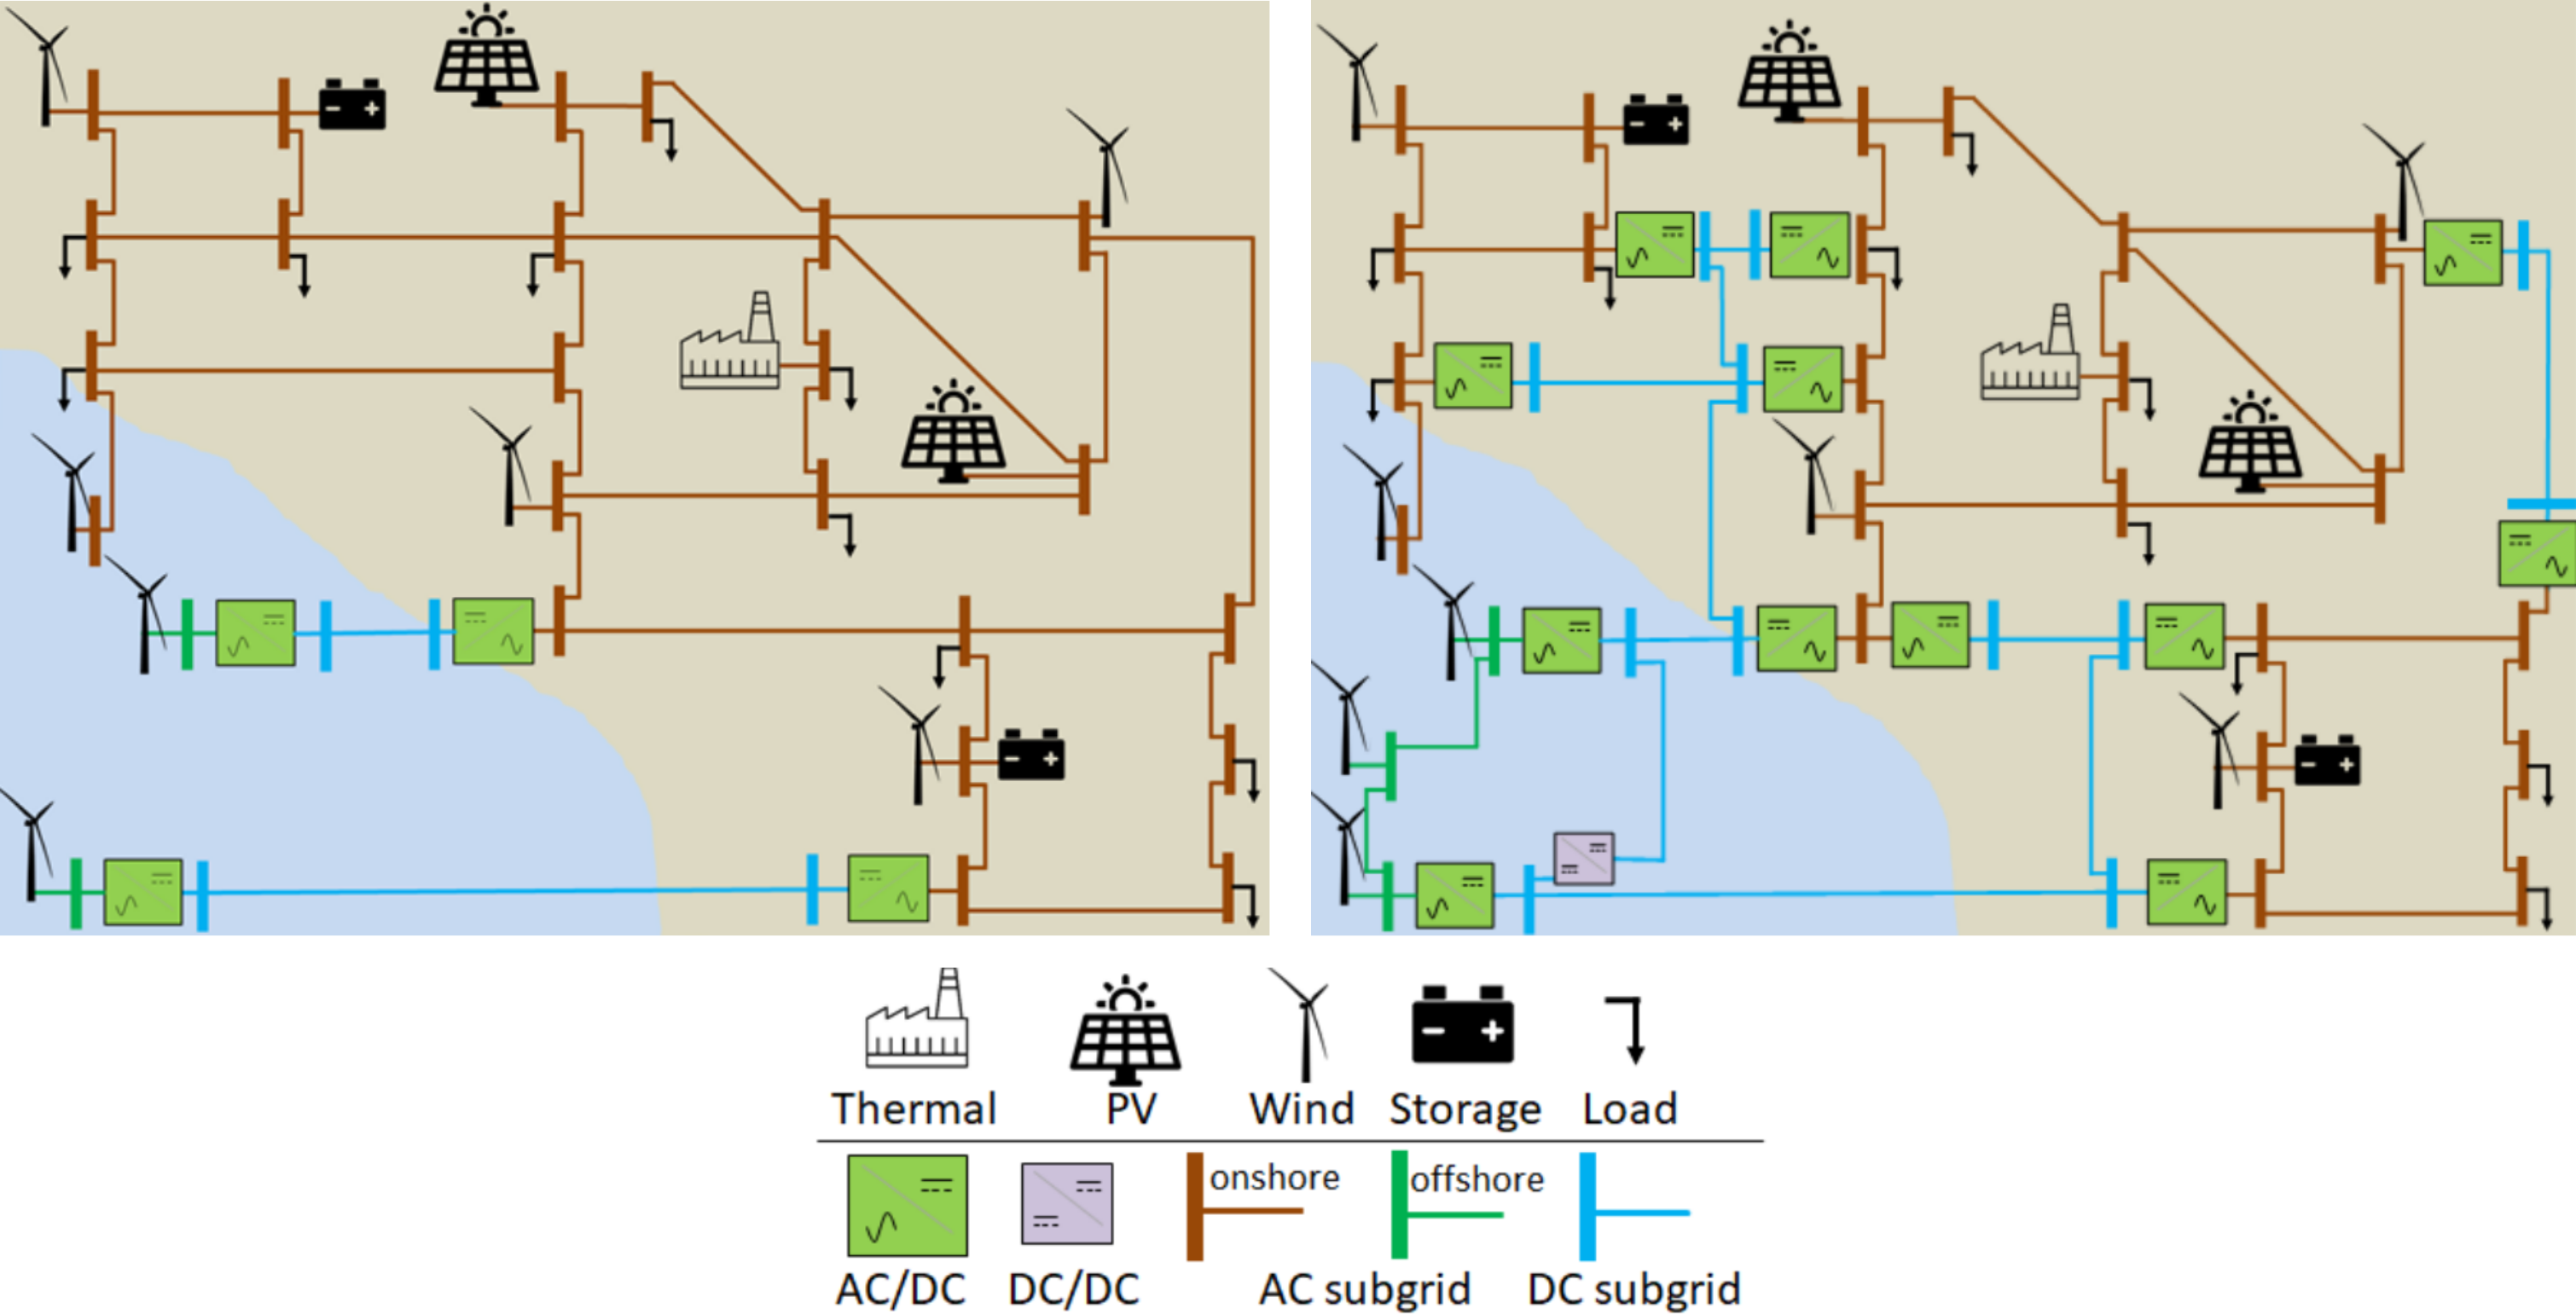
\includegraphics[width=0.9\textwidth]{Images/gridofgrids.png} 
    \caption{From present grids to future systems.}
    \label{fig:gridofgrids}
    \end{figure}
\end{frame}

\subsection{AC/DC converters}
\begin{frame}{Voltage Source Converter (VSC)}
    Voltage source converters (VSCs) interlink AC subsystems with DC subsystems, allowing for controlling two magnitudes. This controllability, while providing more flexibility, also introduces more complexity.
    
    \begin{figure}[!htb]
        \centering
        \begin{circuitikz}[american]
            \draw[line width=0.7mm] (2,0) to [short] (2,-3);
            \draw[line width=0.7mm] (7,0) to [short] (7,-3);
            \draw (2,-1.5) to [sacdc] (7,-1.5);
            \draw (2,-1.5) to [short, i_=$P_t+jQ_t$] (4,-1.5);
            \draw (7,-1.5) to [short, i=$P_f$] (5,-1.5);
            \node at (2,0.35) {$V_t \angle \delta_t$};
            \node at (7,0.35) {$V_f$};
        \end{circuitikz}     
        \caption{Representation of a VSC.}
    \end{figure}
\end{frame}

\begin{frame}{VSC unification of AC and DC sides}
    Converters interconnect DC and AC buses. Hence, there are two approaches to the problem:
    \begin{itemize}
        \item \textbf{Sequential}: we first solve the AC networks, then the DC networks, merge them, and repeat the calculation $\rightarrow$ non-scalable
        \item \textbf{Unified}: we solve all AC and DC grids at the same time $\rightarrow$ much more scalable
    \end{itemize}

    The active powers on the $f$ and $t$ sides are related through the power loss equation:
    \begin{equation}
    \begin{aligned}
        P_f + P_t &= P_{\text{loss}}, \\
        P_f + P_t &= a + b \frac{\sqrt{(P_t)^2 + (Q_t)^2}}{V_t} + c \frac{(P_t)^2 + (Q_t)^2}{V_t^2}. \\
    \end{aligned}
    \end{equation}
\end{frame}


% \subsection{Generalised Branch Model}
% \begin{frame}{Generalised Branch Model}
% \begin{figure}[!htb]
%     \centering
%     \begin{tikzpicture}[european, scale=0.9]

%         % 0. Draw nodes
%         \node(1) at (-0.2, 0) {1};
%         \node(2) at (1.8, -2) {2};
%         \node(3) at (5.0, -2) {3};
%         \node(4) at (5.8, 0) {4};
%         \node(5) at (4.0, 0) {5};
%         \node(6) at (4.0, 1.5) {6};

%         % 1. Draw buses (Passive lines in blue)
%         \draw[line width=0.1cm] (0, 0) to [short] (0.8, 0);
%         \draw[line width=0.1cm] (2, -2) to [short] (2.8, -2);
%         \draw[line width=0.1cm] (6, 0) to [short] (6.8, 0);
%         \draw[line width=0.1cm] (3, 0) to [short] (3.8, 0);
%         \draw[line width=0.1cm] (4, -2) to [short] (4.8, -2);
%         \draw[line width=0.1cm] (3, 1.5) to [short] (3.8, 1.5);

%         % 2. Draw transformers (red circles)
%         \draw[thick, red] (3.4, 0.65) circle (0.2cm);
%         \draw[thick, red] (3.4, 0.85) circle (0.2cm);

%         % 3. Draw generators with additional busbars
%         \draw (0.4, 0.75) to [/tikz/circuitikz/bipoles/length=25pt, sinusoidal voltage source] (0.4, 0.25);
%         \draw (0.4, 0.25) to [short] (0.4, 0); 

%         \draw (2.4, -2.25) to [/tikz/circuitikz/bipoles/length=25pt, sinusoidal voltage source] (2.4, -2.75);
%         \draw (2.4, -2.25) to [short] (2.4, -2.0); 

%         \draw (4.4, -2.25) to [/tikz/circuitikz/bipoles/length=25pt, sinusoidal voltage source] (4.4, -2.75);
%         \draw (4.4, -2.25) to [short] (4.4, -2.0); 

%         % 4. Draw loads
%         \draw (2.1, -2) to [short] (2.1, -2.2);
%         \draw[-{Latex[scale=1.5]}] (2.1,-2.2) -- (1.3,-2.2);

%         \draw (4.7, -2) to [short] (4.7, -2.2);
%         \draw[-{Latex[scale=1.5]}] (4.7,-2.2) -- (5.5,-2.2);

%         \draw (6.8, 0) to [short] (7.0, 0);
%         \draw[-{Latex[scale=1.5]}] (7.0, 0) -- (7.0, -0.8);

%         \draw (3.1, 0) to [short] (3.1, 0.2);
%         \draw[-{Latex[scale=1.5]}] (3.1, 0.2) -- (2.3, 0.2);

%         \draw (3.7, 1.5) to [short] (3.7, 1.7);
%         \draw[-{Latex[scale=1.5]}] (3.7, 1.7) -- (4.5, 1.7);

%         % Draw lines (Passive lines in blue)
%         \draw[blue] (0.4, 0) to [short] (0.4, -0.2);
%         \draw[blue] (2.2, -2) to [short] (2.2, -1.8);
%         \draw[blue] (0.4, -0.2) to [short] (2.2, -1.8);

%         \draw[blue] (0.6, 0) to [short] (0.6, -0.2);
%         \draw[blue] (3.2, 0) to [short] (3.2, -0.2);
%         \draw[blue] (0.6, -0.2) to [short] (3.2, -0.2);

%         \draw[blue] (3.4, 0) to [short] (3.4, -0.2);
%         \draw[blue] (2.4, -2) to [short] (2.4, -1.8);
%         \draw[blue] (3.4, -0.2) to [short] (2.4, -1.8);

%         \draw[blue] (2.6, -2) to [short] (2.6, -2.2);
%         \draw[blue] (4.2, -2) to [short] (4.2, -2.2);
%         \draw[blue] (2.6, -2.2) to [short] (4.2, -2.2);

%         \draw[blue] (2.6, -2) to [short] (2.6, -1.8);
%         \draw[blue] (6.4, 0) to [short] (6.4, -0.2);
%         \draw[blue] (2.6, -1.8) to [short] (6.4, -0.2);

%         \draw[blue] (3.6, 0) to [short] (3.6, -0.2);
%         \draw[blue] (6.2, 0) to [short] (6.2, -0.2);
%         \draw[blue] (3.6, -0.2) to [short] (6.2, -0.2);

%         \draw[blue] (4.4, -2) to [short] (4.4, -1.8);
%         \draw[blue] (6.6, 0) to [short] (6.6, -0.2);
%         \draw[blue] (4.4, -1.8) to [short] (6.6, -0.2);

%         \draw[red] (3.4, 0) to [short] (3.4, 0.45);
%         \draw[red] (3.4, 1.05) to [short] (3.4, 1.5);
%     \end{tikzpicture}
%     \caption{Example grid showing passive lines and active controllable transformer.}
%     \label{fig:14bus}
% \end{figure}



%     In our formulation, we define two sets of branches:
%     \begin{itemize}
%         \item $\kappa$: Passive branches (e.g., lines, non-controllable transformers).
%         \item $\Gamma$: Active branches (e.g., AC/DC interfaces, controllable transformers).
%     \end{itemize}
%     Passive branches ($\kappa$) are reduced to admittances and included in the $Y_\text{bus}$ matrix. Active branches ($\Gamma$) are modeled by power flows through their terminals.
% \end{frame}


% \begin{frame}{Passive Branches}
%     \begin{figure}[!htb]
%         \centering
%         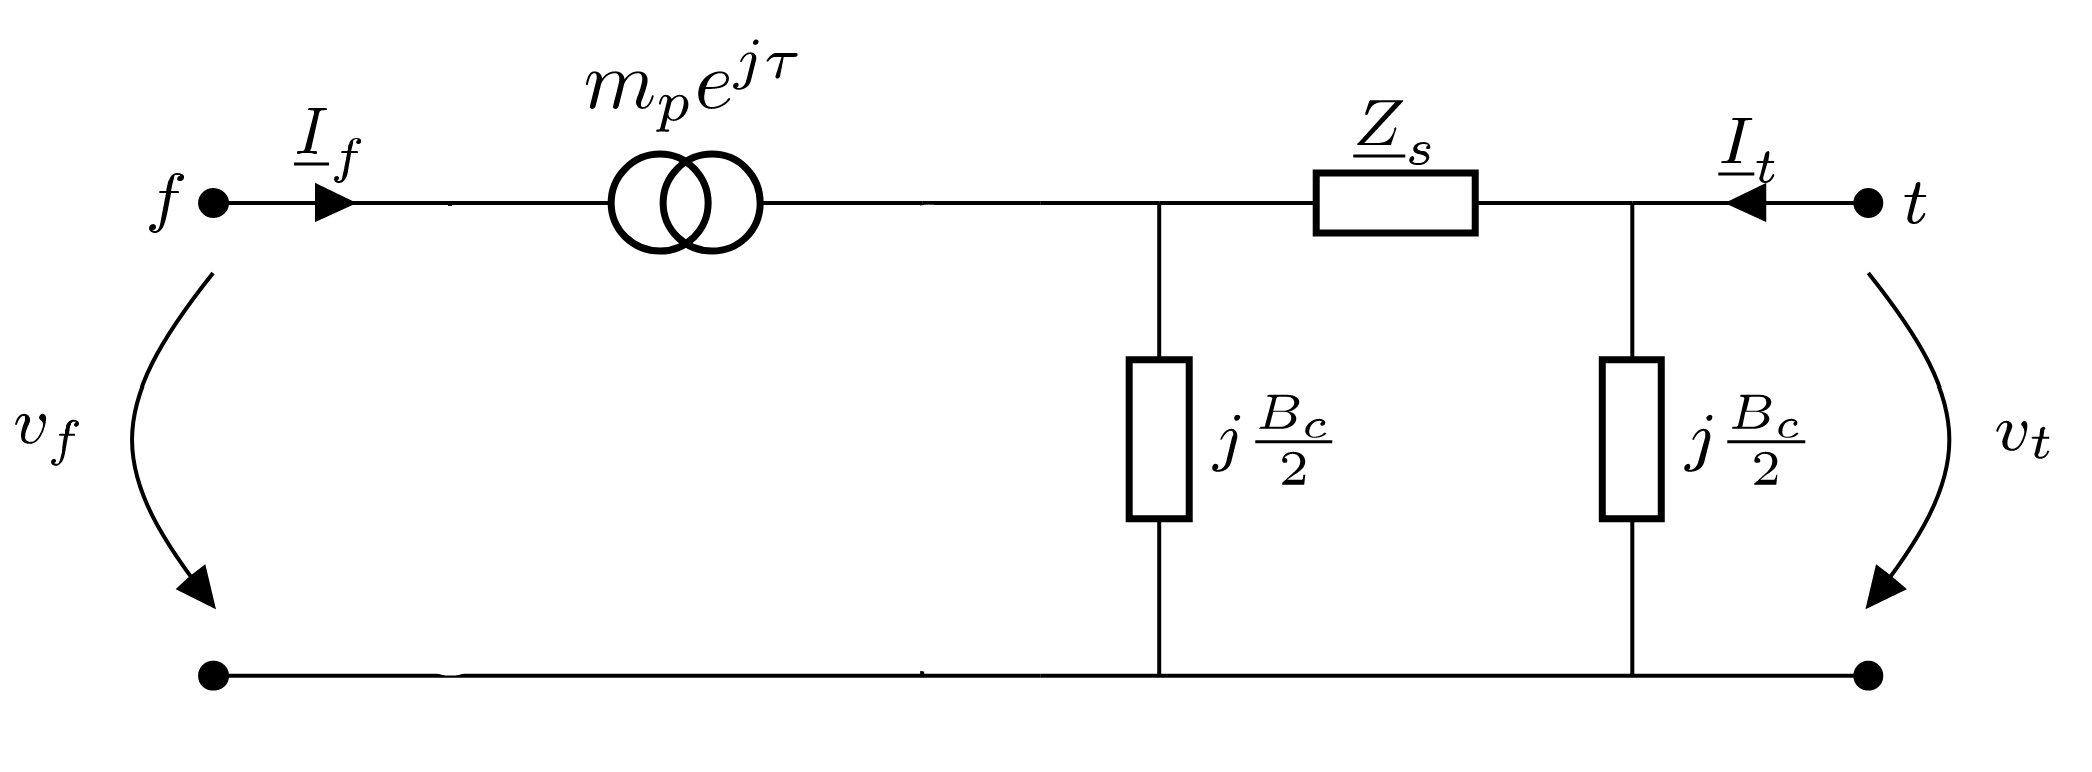
\includegraphics[width=0.6\textwidth]{chapter5pics/branch.png}
%         \caption{Representation of a passive branch.}
%         \label{fig:FUBM}
%     \end{figure} 


%     For any branch $b \in \kappa$ (passive branches), you have a two-by-two admittance matrix:
%     \[
%         Y_{b\in\kappa} = 
%         \begin{bmatrix}
%             Y_{ff} & Y_{ft} \\
%             Y_{tf} & Y_{tt}
%         \end{bmatrix}
%     \]
%     where $Y_{ff}$, $Y_{ft}$, $Y_{tf}$, and $Y_{tt}$ represent the admittance values from the \textit{from} ($f$) and \textit{to} ($t$) sides. The system's $Y_\text{bus}$ matrix is constructed by combining the admittance contributions of all passive branches connected to each bus in the network.
% \end{frame}

% \begin{frame}{FUBM}
%     \begin{figure}[!htb]
%         \centering
%         \includesvg[width=0.6\textwidth]{Images/FUBM.svg}
%         \caption{Flexible Universal Branch Model.}
%         \label{fig:FUBM}
%     \end{figure} 
% The idea of the FUBM is to represent various components in power systems (transmission lines, transformers, and VSCs) in a standardised manner. This model makes no distinction between active and passive branches.

% \end{frame}


% \section{Solving } 

% \begin{frame}{}
%     \tableofcontents[currentsection]
% \end{frame}

\subsection{The power flow}
\begin{frame}{The power flow problem}
    \begin{itemize}
        \item Grid operators are interested in knowing the operating state of the network.
        \item That is, voltages, currents and powers have to be found everywhere in the grid.
        \item The underlying equations, which come from the physics, are non-linear in nature.
        \item Among many solvers, we opt for the Newton-Raphson given its quadratic convergence and scalability properties.
    \end{itemize}

    \begin{equation}
    \bm{x} = [\delta, V, \textcolor{red}{\tau}, \textcolor{red}{m}, \textcolor{red}{P^\text{zip}}, \textcolor{red}{Q^\text{zip}}, \textcolor{red}{P_f}, \textcolor{red}{P_t}, \textcolor{red}{Q_f}, \textcolor{red}{Q_t}]^T
    \end{equation}
    \begin{equation}
    \mathbf{g} =
    [g_{p,ac}, g_{q,ac}, g_{p,dc}, \textcolor{red}{g_{l,acdc}}, \textcolor{red}{g_{l,hvdc}}, \textcolor{red}{g_{p,hvdc}}, \textcolor{red}{g_{p_f,tr}}, \textcolor{red}{g_{p_t,tr}}, \textcolor{red}{g_{q_f,tr}}, \textcolor{red}{g_{q_t,tr}}]^T
    \end{equation}
\end{frame}

\subsection{Solving approach}
\begin{frame}{The Newton-Raphson method}
    \begin{itemize}
    \item To solve the system using the Newton-Raphson method, we need a Jacobian matrix. 
    
    \item This matrix contains the partial derivatives of the form $\frac{\partial{\bm{g}}}{\partial{\bm{x}}}$. Two ways to calculate:
    \begin{enumerate}
        \item Partial differences such as $\frac{\bm{g}(\bm{x} + h) - \bm{g}(\bm{x} - h)}{h}$ $\rightarrow$ easier but slower
        \item With previously derived closed-form expressions $\rightarrow$ harder but faster
    \end{enumerate}
    
    \item The typical Newton-Raphson system is represented as:
    \end{itemize}

    \begin{equation}
        -\mathbf{J} \Delta \mathbf{x} = \mathbf{g}
    \end{equation}
    where:
    \begin{itemize}
        \item $\mathbf{J}$ is the Jacobian matrix.
        \item $\Delta \mathbf{x}$ is the vector of unknown variations.
        \item $\mathbf{g}$ is the residual vector of equations.
    \end{itemize}
\end{frame}

% \begin{frame}{Solving Generalized Power Flow with Newton-Raphson}
%     To solve the generalized power flow problem, a set of known and unknown magnitudes must be defined. 
%     \begin{itemize}
%         \item Known magnitudes are those actively controlled by the system.
%         \item Unknown magnitudes are not directly controlled.
%     \end{itemize}
%     The unknown set $x$ includes:
% \[
% x = [\delta, V, \textcolor{red}{\tau}, \textcolor{red}{m}, \textcolor{red}{P^\text{zip}}, \textcolor{red}{Q^\text{zip}}, \textcolor{red}{P_f}, \textcolor{red}{P_t}, \textcolor{red}{Q_f}, \textcolor{red}{Q_t}]^T
% \]
% \[
% |x| = |\text{DC}|+ 2 \cdot |\text{AC}| + 3 \cdot |\text{VSC}| + 4 \cdot |\text{TR}|
% \]


%     This generalized formulation extends the traditional model by incorporating more unknowns, such as controlled transformers and AC/DC links.
% \end{frame}

% \subsection{Equations and Nodal Balance}
% \begin{frame}{Equations and Nodal Balance (1)}
%     The system of equations must balance the number of unknowns and equations. The nodal balance equations include:
%     \begin{itemize}
%         \item Nodal active and reactive power at AC buses.
%         \item Active power at DC buses.
%         \item Power loss equations for AC/DC links.
%         \item Power equations for controlled transformers.
%         \item Power equations for remotely-controlled passive branches.
%     \end{itemize}
% \end{frame}

% \begin{frame}{Jacobian Variables}
%     The unknown vector $\Delta \mathbf{x}$ is represented as:
%     \[
%     \Delta \mathbf{x} =
%     [\Delta \delta, \Delta V, \Delta \tau, \Delta m, \Delta P^\text{zip}, \Delta Q^\text{zip}, \Delta P_f, \Delta P_t, \Delta Q_f, \Delta Q_t]^T
%     \]
%     The residual vector $\mathbf{g}$ is:
%     \[
%     \mathbf{g} =
%     [g_{p,ac}, g_{q,ac}, g_{p,dc}, g_{p,acdc}, g_{p_f,tr}, g_{p_t,tr}, g_{q_f,tr}, g_{q_t,tr}, g_{p_{ij}, \kappa}, g_{q_{ij}, \kappa}, g_{p_{ji}, \kappa}, g_{q_{ji}, \kappa}]^T
%     \]
% \end{frame}


% \begin{frame}{Jacobian Matrix in Full}
%     \scriptsize  % Shrinks the font size to make it fit better on the slide
%     The full Jacobian matrix $\mathbf{J}$ is constructed as follows, showing the partial derivatives of the equations with respect to the unknown variables:
    
%     \[
%     \mathbf{J} = 
%     \begin{bmatrix}
%         \frac{\partial g_{p,ac}}{\partial \delta} & \frac{\partial g_{p,ac}}{\partial V} & \frac{\partial g_{p,ac}}{\partial \tau} & \frac{\partial g_{p,ac}}{\partial m} & \frac{\partial g_{p,ac}}{\partial P^\text{zip}} & \frac{\partial g_{p,ac}}{\partial Q^\text{zip}} & \frac{\partial g_{p,ac}}{\partial P_f} & \frac{\partial g_{p,ac}}{\partial P_t} & \frac{\partial g_{p,ac}}{\partial Q_f} & \frac{\partial g_{p,ac}}{\partial Q_t} \\
%         \frac{\partial g_{q,ac}}{\partial \delta} & \frac{\partial g_{q,ac}}{\partial V} & \frac{\partial g_{q,ac}}{\partial \tau} & \frac{\partial g_{q,ac}}{\partial m} & \frac{\partial g_{q,ac}}{\partial P^\text{zip}} & \frac{\partial g_{q,ac}}{\partial Q^\text{zip}} & \frac{\partial g_{q,ac}}{\partial P_f} & \frac{\partial g_{q,ac}}{\partial P_t} & \frac{\partial g_{q,ac}}{\partial Q_f} & \frac{\partial g_{q,ac}}{\partial Q_t} \\
%         \frac{\partial g_{p,dc}}{\partial \delta} & \frac{\partial g_{p,dc}}{\partial V} & \frac{\partial g_{p,dc}}{\partial \tau} & \frac{\partial g_{p,dc}}{\partial m} & \frac{\partial g_{p,dc}}{\partial P^\text{zip}} & \frac{\partial g_{p,dc}}{\partial Q^\text{zip}} & \frac{\partial g_{p,dc}}{\partial P_f} & \frac{\partial g_{p,dc}}{\partial P_t} & \frac{\partial g_{p,dc}}{\partial Q_f} & \frac{\partial g_{p,dc}}{\partial Q_t} \\
%         \frac{\partial g_{p,acdc}}{\partial \delta} & \frac{\partial g_{p,acdc}}{\partial V} & \frac{\partial g_{p,acdc}}{\partial \tau} & \frac{\partial g_{p,acdc}}{\partial m} & \frac{\partial g_{p,acdc}}{\partial P^\text{zip}} & \frac{\partial g_{p,acdc}}{\partial Q^\text{zip}} & \frac{\partial g_{p,acdc}}{\partial P_f} & \frac{\partial g_{p,acdc}}{\partial P_t} & \frac{\partial g_{p,acdc}}{\partial Q_f} & \frac{\partial g_{p,acdc}}{\partial Q_t} \\
%         \frac{\partial g_{p_f,tr}}{\partial \delta} & \frac{\partial g_{p_f,tr}}{\partial V} & \frac{\partial g_{p_f,tr}}{\partial \tau} & \frac{\partial g_{p_f,tr}}{\partial m} & \frac{\partial g_{p_f,tr}}{\partial P^\text{zip}} & \frac{\partial g_{p_f,tr}}{\partial Q^\text{zip}} & \frac{\partial g_{p_f,tr}}{\partial P_f} & \frac{\partial g_{p_f,tr}}{\partial P_t} & \frac{\partial g_{p_f,tr}}{\partial Q_f} & \frac{\partial g_{p_f,tr}}{\partial Q_t} \\
%         \frac{\partial g_{p_t,tr}}{\partial \delta} & \frac{\partial g_{p_t,tr}}{\partial V} & \frac{\partial g_{p_t,tr}}{\partial \tau} & \frac{\partial g_{p_t,tr}}{\partial m} & \frac{\partial g_{p_t,tr}}{\partial P^\text{zip}} & \frac{\partial g_{p_t,tr}}{\partial Q^\text{zip}} & \frac{\partial g_{p_t,tr}}{\partial P_f} & \frac{\partial g_{p_t,tr}}{\partial P_t} & \frac{\partial g_{p_t,tr}}{\partial Q_f} & \frac{\partial g_{p_t,tr}}{\partial Q_t} \\
%         \frac{\partial g_{q_f,tr}}{\partial \delta} & \frac{\partial g_{q_f,tr}}{\partial V} & \frac{\partial g_{q_f,tr}}{\partial \tau} & \frac{\partial g_{q_f,tr}}{\partial m} & \frac{\partial g_{q_f,tr}}{\partial P^\text{zip}} & \frac{\partial g_{q_f,tr}}{\partial Q^\text{zip}} & \frac{\partial g_{q_f,tr}}{\partial P_f} & \frac{\partial g_{q_f,tr}}{\partial P_t} & \frac{\partial g_{q_f,tr}}{\partial Q_f} & \frac{\partial g_{q_f,tr}}{\partial Q_t} \\
%         \frac{\partial g_{q_t,tr}}{\partial \delta} & \frac{\partial g_{q_t,tr}}{\partial V} & \frac{\partial g_{q_t,tr}}{\partial \tau} & \frac{\partial g_{q_t,tr}}{\partial m} & \frac{\partial g_{q_t,tr}}{\partial P^\text{zip}} & \frac{\partial g_{q_t,tr}}{\partial Q^\text{zip}} & \frac{\partial g_{q_t,tr}}{\partial P_f} & \frac{\partial g_{q_t,tr}}{\partial P_t} & \frac{\partial g_{q_t,tr}}{\partial Q_f} & \frac{\partial g_{q_t,tr}}{\partial Q_t} \\
%         \frac{\partial g_{pf, \kappa }}{\partial \delta} & \frac{\partial g_{pf, \kappa }}{\partial V} & \frac{\partial g_{pf, \kappa }}{\partial \tau} & \frac{\partial g_{pf, \kappa }}{\partial m} & \frac{\partial g_{pf, \kappa }}{\partial P^\text{zip}} & \frac{\partial g_{pf, \kappa }}{\partial Q^\text{zip}} & \frac{\partial g_{pf, \kappa }}{\partial P_f} & \frac{\partial g_{pf, \kappa }}{\partial P_t} & \frac{\partial g_{pf, \kappa }}{\partial Q_f} & \frac{\partial g_{pf, \kappa }}{\partial Q_t} \\
%         \frac{\partial g_{qf, \kappa }}{\partial \delta} & \frac{\partial g_{qf, \kappa }}{\partial V} & \frac{\partial g_{qf, \kappa }}{\partial \tau} & \frac{\partial g_{qf, \kappa }}{\partial m} & \frac{\partial g_{qf, \kappa }}{\partial P^\text{zip}} & \frac{\partial g_{qf, \kappa }}{\partial Q^\text{zip}} & \frac{\partial g_{qf, \kappa }}{\partial P_f} & \frac{\partial g_{qf, \kappa }}{\partial P_t} & \frac{\partial g_{qf, \kappa }}{\partial Q_f} & \frac{\partial g_{qf, \kappa }}{\partial Q_t} \\
%         \frac{\partial g_{pt, \kappa }}{\partial \delta} & \frac{\partial g_{pt, \kappa }}{\partial V} & \frac{\partial g_{pt, \kappa }}{\partial \tau} & \frac{\partial g_{pt, \kappa }}{\partial m} & \frac{\partial g_{pt, \kappa }}{\partial P^\text{zip}} & \frac{\partial g_{pt, \kappa }}{\partial Q^\text{zip}} & \frac{\partial g_{pt, \kappa }}{\partial P_f} & \frac{\partial g_{pt, \kappa }}{\partial P_t} & \frac{\partial g_{pt, \kappa }}{\partial Q_f} & \frac{\partial g_{pt, \kappa }}{\partial Q_t} \\
%         \frac{\partial g_{qt, \kappa }}{\partial \delta} & \frac{\partial g_{qt, \kappa }}{\partial V} & \frac{\partial g_{qt, \kappa }}{\partial \tau} & \frac{\partial g_{qt, \kappa }}{\partial m} & \frac{\partial g_{qt, \kappa }}{\partial P^\text{zip}} & \frac{\partial g_{qt, \kappa }}{\partial Q^\text{zip}} & \frac{\partial g_{qt, \kappa }}{\partial P_f} & \frac{\partial g_{qt, \kappa }}{\partial P_t} & \frac{\partial g_{qt, \kappa }}{\partial Q_f} & \frac{\partial g_{qt, \kappa }}{\partial Q_t}
%     \end{bmatrix}
%     \]
% \end{frame}




\begin{frame}{Rules for solvability}
    \begin{columns}
        % Left column with the rules
        \begin{column}{0.5\textwidth}
            To ensure solvability in generalized power flow, the following rules are defined:
            \begin{itemize}
                \item Each subgrid must have at least one reference for voltage magnitude and angle.
                \item Control of a remote bus is allowed.
                \item No two devices can control the same nodal voltage.
                \item Buses can have up to 4 controlled magnitudes in AC subsystems and 2 in DC subsystems.
            \end{itemize}
        \end{column}
        
        % Right column with the figure
        \begin{column}{0.5\textwidth}
            \begin{figure}[H]
                \centering
                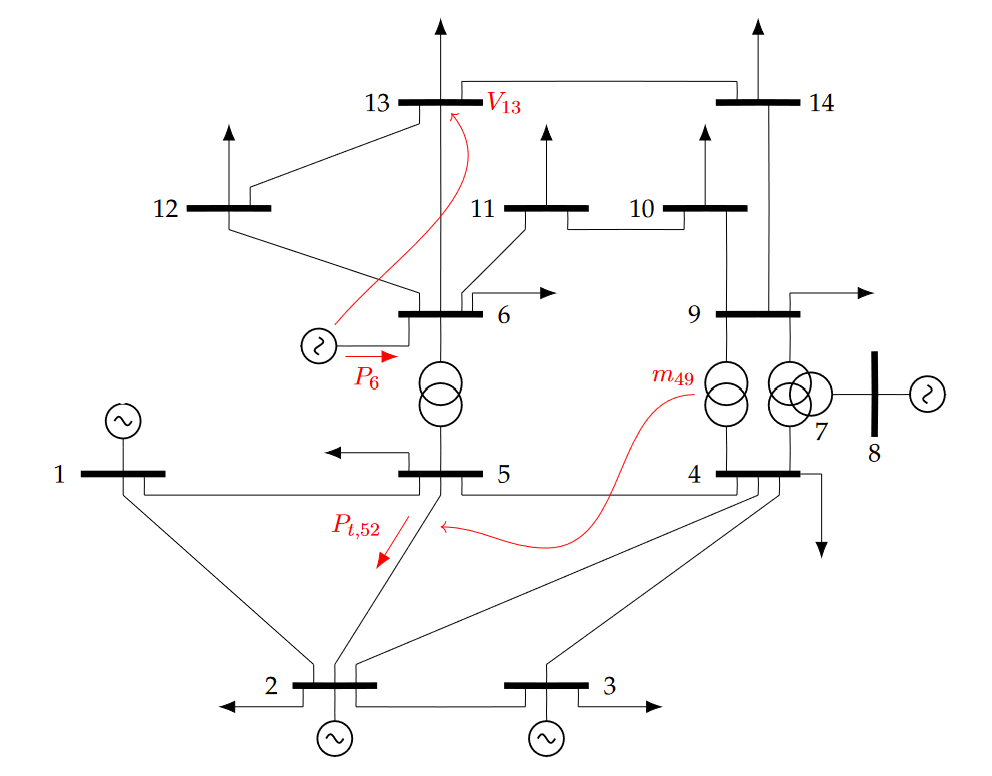
\includegraphics[width=0.9\textwidth]{chapter5pics/remote.png}
                \caption{Scheme of the IEEE 14-bus grid with remote controls.}
                \label{fig:simple6bus}
            \end{figure}
        \end{column}
    \end{columns}
\end{frame}



